\section{Ge}
\subsection*{Material ID: mp-bg}
\textbf{Constante Dieléctrica ($\epsilon_{total}$):} 25.85 \\[0.5em]
\begin{table}[h!]
\centering
\begin{tabular}{lcc}
\toprule
\textbf{Métrica} & \textbf{Lámina (Plate)} & \textbf{Cilindros (Rod)} \\
\midrule
Bandgaps ($a/\lambda$) & Ninguno & Ninguno \\
Resonancias & 36 & 36 \\
\bottomrule
\end{tabular}
\end{table}
\begin{figure}[H]
\centering
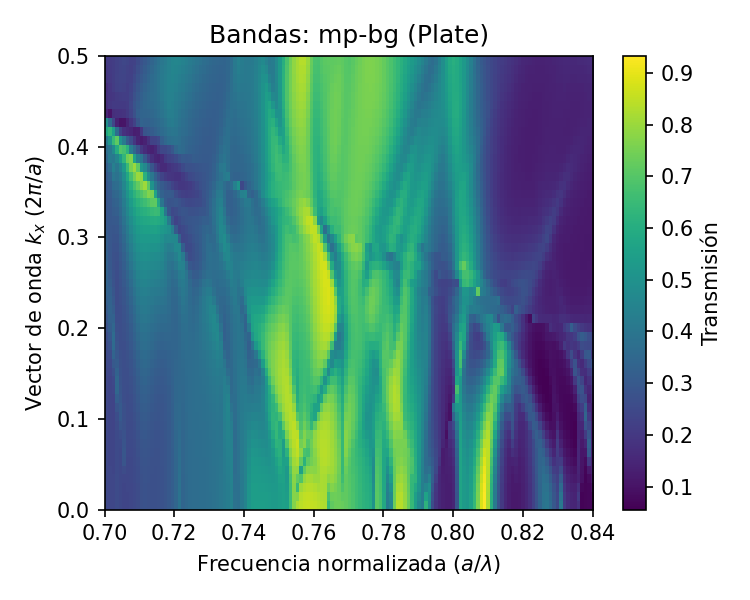
\includegraphics[width=0.48\textwidth]{figures/mp-bg_plate.png}
\hfill
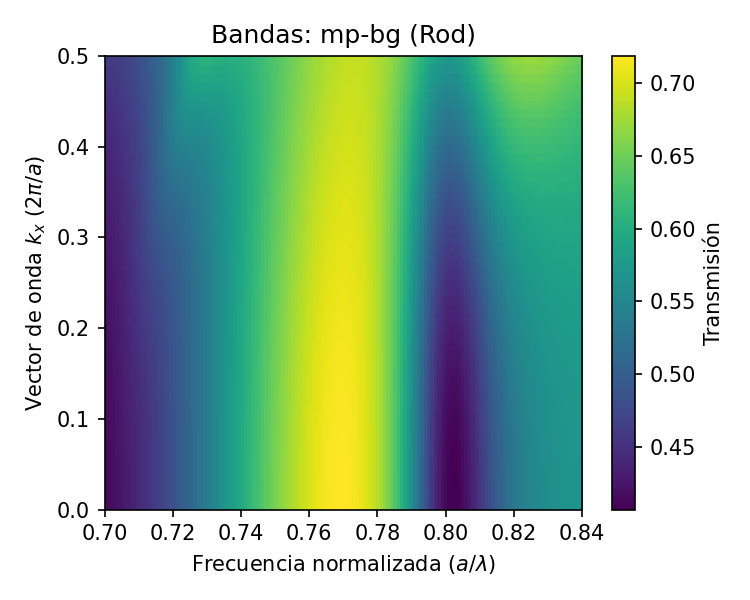
\includegraphics[width=0.48\textwidth]{figures/mp-bg_rod.png}
\caption{Estructuras de bandas fotónicas para mp-bg. Izquierda: Lámina. Derecha: Cilindros.}
\end{figure}
\vspace{1em}
\hrule
\vspace{1em}
\subsection*{Material ID: mp-fh}
\textbf{Constante Dieléctrica ($\epsilon_{total}$):} 40.19 \\[0.5em]
\begin{table}[h!]
\centering
\begin{tabular}{lcc}
\toprule
\textbf{Métrica} & \textbf{Lámina (Plate)} & \textbf{Cilindros (Rod)} \\
\midrule
Bandgaps ($a/\lambda$) & [0.733 - 0.734] & Ninguno \\
Resonancias & 36 & 36 \\
\bottomrule
\end{tabular}
\end{table}
\begin{figure}[H]
\centering
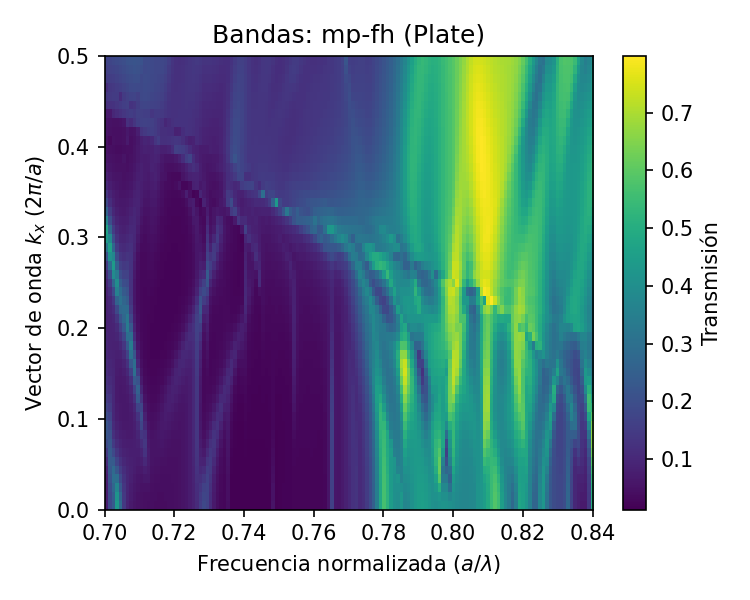
\includegraphics[width=0.48\textwidth]{figures/mp-fh_plate.png}
\hfill
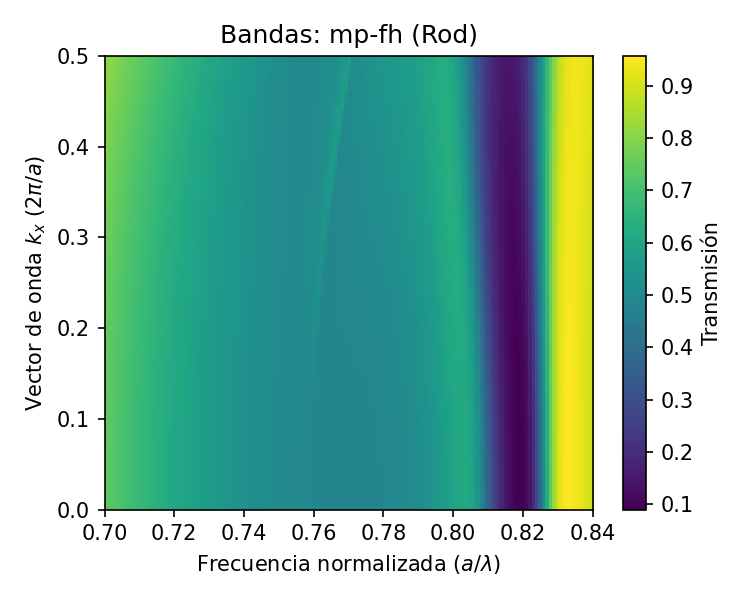
\includegraphics[width=0.48\textwidth]{figures/mp-fh_rod.png}
\caption{Estructuras de bandas fotónicas para mp-fh. Izquierda: Lámina. Derecha: Cilindros.}
\end{figure}
\vspace{1em}
\hrule
\vspace{1em}

\subsection*{Analisis}

Un material con un gap detectado automaticamente!!! Eso es bastante valioso pues permite encontra que en ese gap concreto no se deberia transmitir al recrear las condiciones planteadas (o al menos se deberia reducir considerablemente la transmision). Ademas como ya es comun el material lo encontre en esta misma web \url{https://order.universitywafer.com/default.aspx?cat=Germanium} aunque este es considerablemente mas costoso que los anteriores. Ademas, para ser honesto este es un resultado en el que no confio pues los valores reportados en MP son inmensos (bastante mayores de lo que tendria sentido). Aun no entiendo bien por que los reportes concretos en la base de datos que busque fallaron pero provare con otros valores para confirmarlo.

\clearpage
